\section{ADC}
\subsection{Purpose of the ADC}
An ADC converter is needed for this project to convert the analog voltages which the photo diode create into an digital value which the digital logic need to determine the color of the block.   
The ADC component being used for this process will be the MCP3008, which is an 10 bit ADC converter.  
\subsection{MCP3008}
The MCP3008 is an ADC component, it is capable of converting an analog value from the ranging from 2.7 - 5.5 into an 10 bit value. It is rated to have an conversion rate of 200 ksps at an $V_{dd} = 5V$


\todo[inline]{\textbf{-- Billede af komponentn\\
}}

\begin{figure}[H]
\center
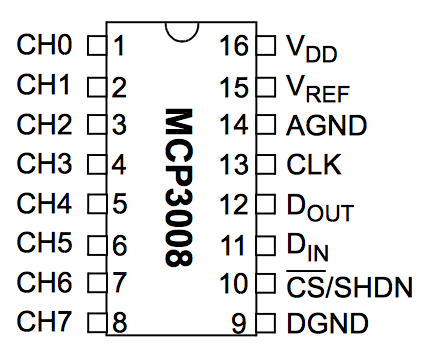
\includegraphics[scale = 0.5]{images/MPC3008.png}
\caption{}
\end{figure}
The chip has 16 pins, at which the pins to the left consist of 8 seperate input ports for analog voltages, and the right side consist of V\textsubscript{dd}, V\textsubscript{ref}, AGND , CLK, CS, Dout,  Din.   The FPGA interfaces the with ADC using the pins CLK, CS, DOUT, DIN. 
The ADC uses an SPI-based interface to communicate with the FPGA. \\


The CLK consist of the clock frequency at which data will be sent to the ADC and read from the ADC. According to the datasheet is the max frequency for the comunication 3.57 mHz, which the FPGA provides it with at that port. The datasheet states that the min. clock rate has to be 10Khz as this will affect the linearity performance of the ADC,  and especially as different temperatures. \\


Din is the input port which the FPGA sends the init bits to. 
As the component is only going to read an analog value from CHO, and convert into a digital value,  will the init bits send to the ADC be "11000".  The first '1' is the start bit ,  The next '1' bit bit determines whether the system should perform a single ended or differential conversion. Single ended conversion converts the input from one port, and differential conversion converts the difference between two ports. '1' declares the conversion as an single ended conversion. The last 3 bits "000" determines the port at which it has to read from, in this case it is always from CH0. The init bits can either be send at either the rising or falling edge of the clock.   \\
  

Dout is the output port which the FPGA reads the converted analog value as an 10 bit digital binary number. When a conversion has been performed,  the first bit the which will be read from the Dout port will be the a null bit, and afterwards will each bit of the 10 bit be outputted from MSB to LSB. Dout will stay undefined, until the init bits has been provided to the port, and the sample and hold period has passed being 1.5 clockcycle according to the datasheet. Due to this sample and hold period, will the output be clocked out,  on the inverse clockevent of the init bits were sent.\\


CS is chip select. It is used to initiate communication between ADC and FPGA, when it is pulled low, when it is pulled high, it will end the conversion and put the ADC in a standby mode.  It must be pulled high between each new conversions. 
 


\todo[inline]{\textbf{-- diagram viser timing tingen -- \\
}}
\subsection{Implementation of communication}

The communication between MPC3008 and the FPGA is implemented as an entity named ADC. The communication is implemented based on the timing diagram as showed in \ref{fig:ADC_diagram} .  A conversion  consist of 17 rising edge clock event.  \\

As the component operates on a lower clock frequency than the FPGA provides. A process named \texttt{prescaler01}, changes the state of the signal \texttt{newClock} with an frequency of $3.57$ Mhz. \\

Within another process called \texttt{ADC\_states},  a variable named \texttt{clockCount} is incremented for each rising edge of \texttt{newClock}.  Within this process  both \texttt{falling\_edge} and \texttt{rising\_edge} of \texttt{newClock} is detected. \\

When \texttt{clockCount} is between 0 and 1 on a \texttt{falling\_edge} of the \texttt{newClock}, the \texttt{CS} is set high, \texttt{MOSI} is set low, and \texttt{read\_adc} is low such that other components connected that the binary output is not ready to be read. \\

When \texttt{clockCount} is between 1 and 5 on a \texttt{falling\_edge} of the \texttt{newClock}, will the \texttt{CS} be set low, and send  these bits "11000" from msb to lsb while \texttt{clockCount} is between 1 and 5, using  the MOSI.  \\

When \texttt{clockCount} is 6 on a \texttt{falling\_edge} of the \texttt{newClock} will MOSI  set to low. At this state MPC3008 start its sample and time. \\



When \texttt{clockCount} is between 6 and 8 on a \texttt{rising\_edge} of the \texttt{newClock} will MOSI still be low, MPC3008  will still be sampling and at the eight clockCount it would have outputted  a NULL bit. \\

When \texttt{clockCount} is between 8  and 18 on a \texttt{rising\_edge} of the \texttt{newClock}, is RX concatenated 10 times with MISO, which read the each bit the MCP3008 outputs.\\

When \texttt{clockCount} is 18 on a \texttt{falling\_edge} of the \texttt{newClock} is \texttt{read\_adc} set high, such that other component conected that that pin will know that the adc value is ready to be read from. \\

When \texttt{clockCount} is 19 on \texttt{rising\_edge} of the \texttt{newClock} is \texttt{clockCount} set to zero, everything start all over again. \\

The conversion itself take up 17 \texttt{rising\_edges} and one \texttt{clockCount} is used to set \texttt{CS} high ,  and one \texttt{clockCount} is used to make sure that it read the 10 bit value. 


%begin{figure}[htb]
%\centering
%\begin{tikzpicture}[font=\sffamily,>=triangle 45]
%  \node [shape=circuit] (item) at (0,0) {adc};
%  \draw [<-] (item.ina) node [anchor=west,labels] {} -- +(-1,0) node [anchor=east] {MISO};
%  \draw [->] (item.outa) node [anchor=east,labels] {} -- +(1,0) node [anchor=west] {MOSI};
%  \draw [->] (item.outb) node [anchor=east,labels] {} -- +(1,0) node [anchor=west] {CS};
%  \draw [->] (item.outc) node [anchor=east,labels] {} -- +(1,0) node [anchor=west] {SCLK};
%  \draw [<-] (item.inb) node [anchor=west,labels] {} -- +(-1,0) node [anchor=east] {CLK};
%  \draw [->] (item.outd) node [anchor=east,labels] {} -- +(1,0) node [anchor=west] {read\_adc};
%  \draw [<-] (item.inc) node [anchor=west,labels] {} -- +(-1,0) node [anchor=east] {start\_adc};
%  \draw [->] (item.oute) node [anchor=east,labels] {} -- +(1,0) node [anchor=west] {ADC\_value};
%\end{tikzpicture}
%\caption{Entity of adc}
%\end{figure}

\subsection{Logic Level Converters}
When supplied with 5V, the MCP3008 uses TTL for communication while the FPGA uses 3.3V CMOS. To protect the FPGA it is necessary to translate the logic high of TTL, $V_h=5V$, to logic high of CMOS, $V_h=3.3V$. In order to achieve this a simple circuit was utilized. See figure \ref{circ:logiclevel}. 
<<<<<<< HEAD
%\begin{figure}
%	\begin{circuitikz}
%		\draw(0,0)
%			\to[R] ++(0,2)
%	;\end{circuitikz}
%\end{figure}  
=======
\begin{figure}
	\begin{circuitikz}
%		\draw(0,0)
%			\to[R] ++(0,2)
	;\end{circuitikz}
\end{figure}  
